\documentclass[tikz,border=3pt]{standalone}
\usepackage{ctex}
\usepackage{tikz}
\usetikzlibrary{calc,arrows.meta}

\tikzset{
	axis/.style={thick,->,>=Stealth},
	vec/.style={thick,->,>=Stealth},
	aux/.style={thin,dashed},
	err/.style={blue!70!black,thick,->,>=Stealth},
	pt/.style={circle,fill=black,inner sep=1.2pt}
}

\begin{document}
	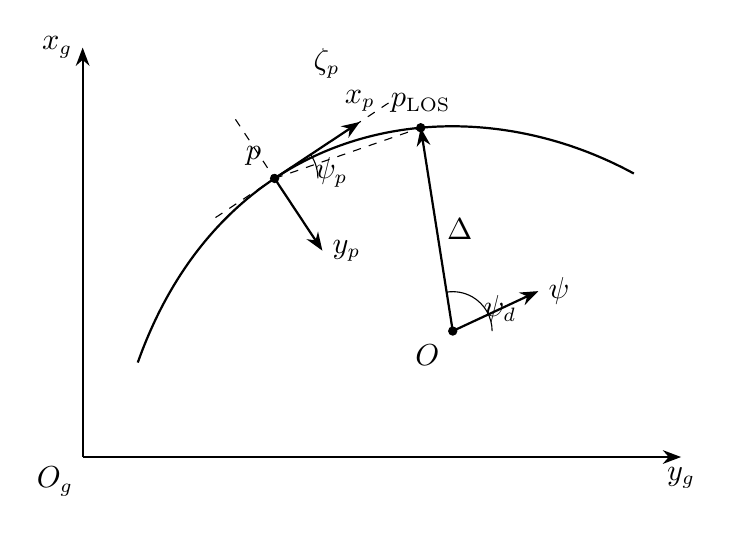
\begin{tikzpicture}[font=\songti\fontsize{10.5pt}{12pt}\selectfont]
		
		% -------------------------------------------------
		% 1. Global axes (page coordinates: x right, y up;
		%    only labels are swapped to match thesis notation)
		% -------------------------------------------------
		\coordinate (Og) at (0,0);
		\draw[axis] (Og) -- (0,5.2) node[left] {$x_g$};
		\draw[axis] (Og) -- (7.6,0) node[below] {$y_g$};
		\node[below left] at (Og) {$O_g$};
		
		% -------------------------------------------------
		% 2. Cubic Bezier control points
		% -------------------------------------------------
		\coordinate (P0) at (0.7,1.2);
		\coordinate (P1) at (1.8,4.3);
		\coordinate (P2) at (4.8,4.8);
		\coordinate (P3) at (7.0,3.6);
		
		% Draw reference path
		\draw[thick] (P0) .. controls (P1) and (P2) .. (P3);
		\node at (3.1,5.0) {$\zeta_p$};
		
		% -------------------------------------------------
		% 3. Choose path parameter for projection point p
		% -------------------------------------------------
		\pgfmathsetmacro{\tp}{0.35}
		\pgfmathsetmacro{\tlos}{0.62}
		
		% Bezier point p = B(tp)
		\pgfmathsetmacro{\Px}{
			(1-\tp)^3*(0.7)
			+ 3*(1-\tp)^2*\tp*(1.8)
			+ 3*(1-\tp)*\tp^2*(4.8)
			+ \tp^3*(7.0)
		}
		\pgfmathsetmacro{\Py}{
			(1-\tp)^3*(1.2)
			+ 3*(1-\tp)^2*\tp*(4.3)
			+ 3*(1-\tp)*\tp^2*(4.8)
			+ \tp^3*(3.6)
		}
		
		% Bezier point p_LOS = B(tlos)
		\pgfmathsetmacro{\Plx}{
			(1-\tlos)^3*(0.7)
			+ 3*(1-\tlos)^2*\tlos*(1.8)
			+ 3*(1-\tlos)*\tlos^2*(4.8)
			+ \tlos^3*(7.0)
		}
		\pgfmathsetmacro{\Ply}{
			(1-\tlos)^3*(1.2)
			+ 3*(1-\tlos)^2*\tlos*(4.3)
			+ 3*(1-\tlos)*\tlos^2*(4.8)
			+ \tlos^3*(3.6)
		}
		
		\coordinate (P) at (\Px,\Py);
		\coordinate (Plos) at (\Plx,\Ply);
		
		% -------------------------------------------------
		% 4. Exact tangent at p : B'(tp)
		% -------------------------------------------------
		\pgfmathsetmacro{\Tx}{
			3*(1-\tp)^2*(1.8-0.7)
			+ 6*(1-\tp)*\tp*(4.8-1.8)
			+ 3*\tp^2*(7.0-4.8)
		}
		\pgfmathsetmacro{\Ty}{
			3*(1-\tp)^2*(4.3-1.2)
			+ 6*(1-\tp)*\tp*(4.8-4.3)
			+ 3*\tp^2*(3.6-4.8)
		}
		
		% Tangent norm
		\pgfmathsetmacro{\Tnorm}{veclen(\Tx,\Ty)}
		
		% Unit tangent
		\pgfmathsetmacro{\tx}{\Tx/\Tnorm}
		\pgfmathsetmacro{\ty}{\Ty/\Tnorm}
		
		% Right normal (clockwise 90 deg)
		\pgfmathsetmacro{\nx}{\ty}
		\pgfmathsetmacro{\ny}{-\tx}
		
		% Tangent angle
		\pgfmathsetmacro{\psip}{atan2(\Ty,\Tx)}
		
		% -------------------------------------------------
		% 5. Path point and local path frame
		% -------------------------------------------------
		\node[pt,label=above left:$p$] at (P) {};
		\node[pt,label=above:$p_{\mathrm{LOS}}$] at (Plos) {};
		
		% x_p along tangent
		\draw[vec] (P) -- ++({1.3*\tx},{1.3*\ty}) node[above] {$x_p$};
		
		% y_p along right normal
		\draw[vec] (P) -- ++({1.1*\nx},{1.1*\ny}) node[right] {$y_p$};
		
		% auxiliary tangent / normal lines
		\draw[aux] ($(P)+({-0.9*\tx},{-0.9*\ty})$) -- ($(P)+({1.8*\tx},{1.8*\ty})$);
		\draw[aux] ($(P)+({-0.9*\nx},{-0.9*\ny})$) -- ($(P)+({1.0*\nx},{1.0*\ny})$);
		
		% psi_p angle (relative to page x-axis, but labeled as path heading)
		\draw ($(P)+(0.55,0)$) arc[start angle=0,end angle=\psip,radius=0.55];
		\node at ($(P)+(0.72,0.08)$) {$\psi_p$};
		
		% -------------------------------------------------
		% 6. Vessel position
		% -------------------------------------------------
		\coordinate (O) at (4.7,1.6);
		\node[pt,label=below left:$O$] at (O) {};
		
		% simple LOS line
		\draw[vec] (O) -- (Plos) node[midway,right] {$\Delta$};
		
%		% cross-track style auxiliary
%		\draw[aux] (P) -- (O);
%		\draw[err] ($(P)+(-0.08,-0.08)$) -- ($(O)+(-0.10,0.10)$)
%		node[midway,left] {$e_y$};
		
		% desired heading angle psi_d from horizontal to LOS
		\pgfmathanglebetweenpoints{\pgfpointanchor{O}{center}}{\pgfpointanchor{Plos}{center}}
		\let\psid\pgfmathresult
		\draw ($(O)+(0.5,0)$) arc[start angle=0,end angle=\psid,radius=0.5];
		\node at ($(O)+(0.60,0.28)$) {$\psi_d$};
		
		% draw actual heading psi
		\draw[vec] (O) -- ++(25:1.2) node[right] {$\psi$};
		
		% path segment from p to p_LOS
		\draw[aux] (P) -- (Plos);
		
	\end{tikzpicture}
\end{document}